\chapter{Fachklassenmodell}\label{ch:fachklassenmodell}


\section{Beziehungsdiagramm}\label{sec:beziehungsdiagramm}
Im folgenden Beziehungsdiagramm (Abbildung~\ref{fig:beziehungsdiagramm}) sind die Beziehungen zwischen den einzelnen Klassen dargestellt.

\begin{figure}[H]
    \centering
    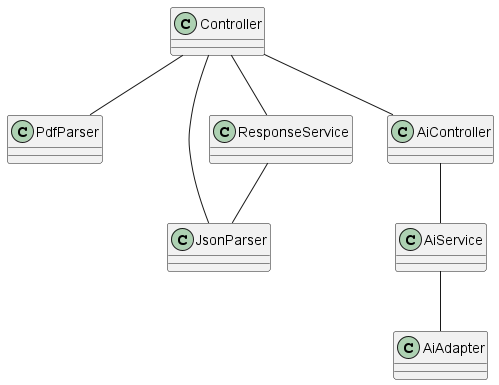
\includegraphics[width=0.75\textwidth]{images/diagrams/Beziehungsdiagramm}
    \caption{Beziehungsdiagramm}
    \label{fig:beziehungsdiagramm}
\end{figure}


\section{Fachklassendiagramm}\label{sec:fachklassendiagramm}
\begin{figure}[H]
    \centering
    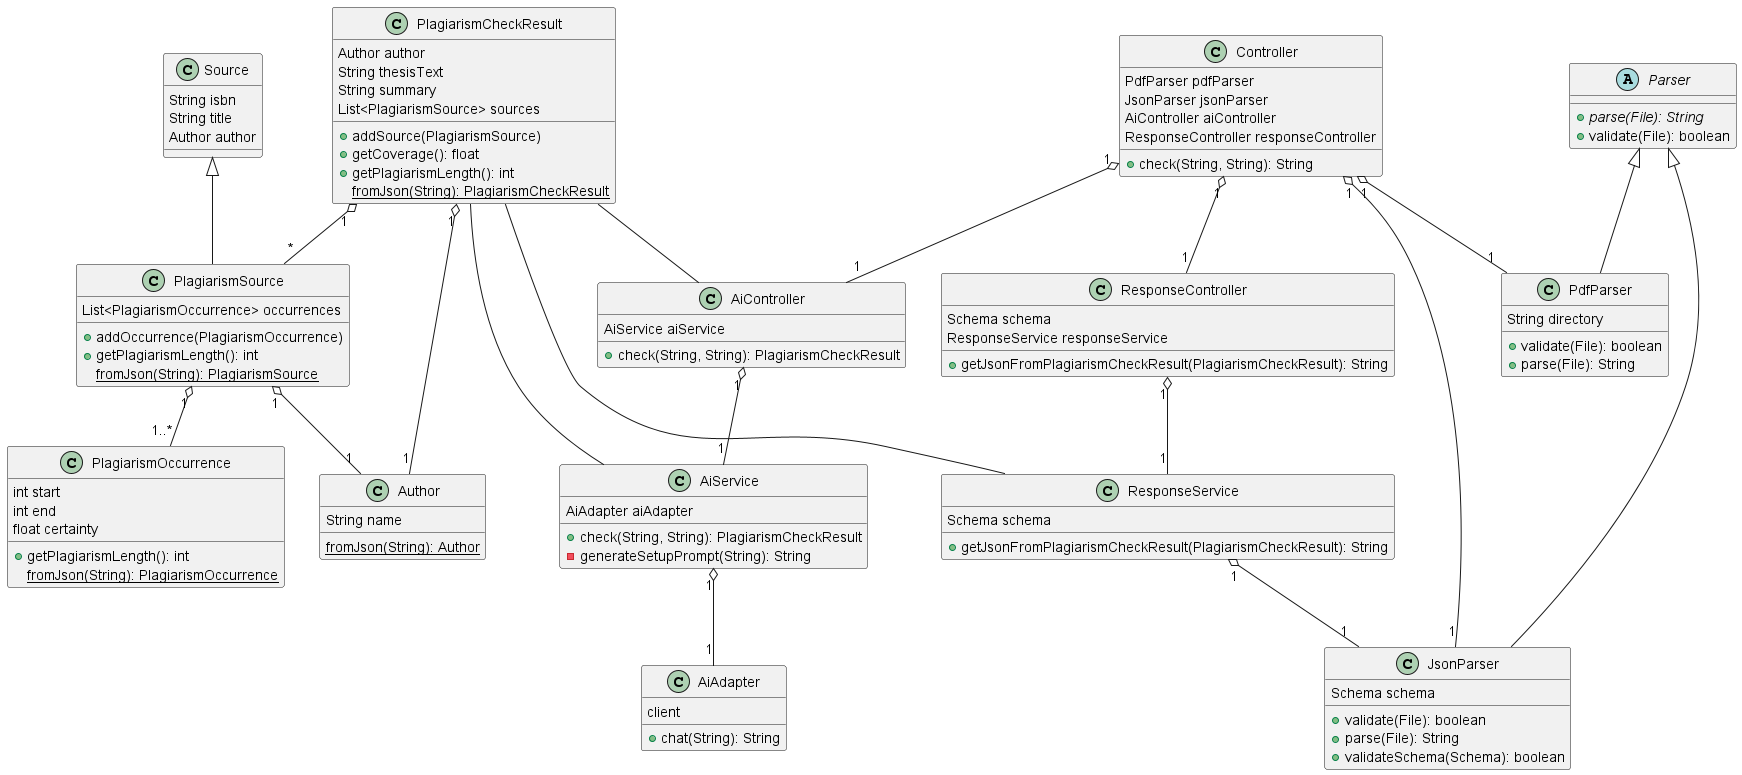
\includegraphics[width=\textwidth]{images/diagrams/Klassendiagramm}
    \caption{Fachklassendiagramm}
    \label{fig:fachklassendiagramm}
\end{figure}


\section{Beschreibung der Fachklassen}\label{sec:beschreibung_der_fachklassen}

\subsection{Controller}\label{subsec:controller}
Dies ist die Hauptsteuerungsklasse,
sie ist verantwortlich für die Abwicklung der Anfragen und Antworten in der Anwendung.
Der Controller enthält außerdem die an die Schnittstelle gesendeten Anfragen und koordiniert die Kommunikation zwischen den einzelnen Diensten.

\subsection{Author}\label{subsec:author}
Die Author-Klasse stellt einen Autor dar und enthält den Namen des Autors.
In unserem System repräsentiert sie den Autor einer Bachelorarbeit oder den Autor einer Quelle.

\subsection{Source}\label{subsec:source}
Die Source-Klasse stellt eine Quelle dar.
Sie entspricht einem Buch, einer Webseite oder einem anderen Dokument aus der realen Welt.
Sie enthält Informationen über den Autor, den Titel und die ISBN der Quelle.

\subsection{PlagiarismCheck}\label{subsec:plagiarism_check}

\subsubsection{PlagiarismCheckResult}\label{subsubsec:plagiarism_check_result}
Diese Klasse wird verwendet, um das von der KI gesendete Ergebnis der Überprüfung in einem einheitlichen Format zu halten.
Sie enthält eine Liste von PlagiarismSources, die die Quellen des Plagiats darstellen.
Zudem enthält sie eine Kurzzusammenfassung des Ergebnisses der Überprüfung,
den Autor und den Inhalt der Bachelorarbeit.

\subsubsection{PlagiarismOccurrence}\label{subsubsec:plagiarism_occurrence}
Dieses Modell repräsentiert eine einzelne Quelle eines möglichen Plagiats.
Es enthält Informationen über die ISBN, den Titel,
den Autor der Quelle, und die Stellen, an denen das Plagiat aufgetreten ist.

\subsubsection{PlagiarismSource}\label{subsubsec:plagiarism_source}
Diese Klasse erweitert die Source-Klasse um die Informationen, die für die Plagiatsprüfung benötigt werden.
Eine solche Information ist beispielsweise eine Liste mit Stellen im Text, die der Quelle zugeordnet werden können.
Auch zusätzliche Funktionalität wie die Anzahl der Zeichen, die für diese Quelle als Plagiat im Text markiert wurden,
wird in dieser Klasse implementiert.

\subsection{AI}\label{subsec:ai}

\subsubsection{AiController}\label{subsubsec:ai_controller}
Der AiController verwaltet den AiService und dient der Koordination aller Abläufe,
welche mit der Anfrage an das verwendete KI-System zusammenhängen.

\subsubsection{AiService}\label{subsubsec:ai_service}
Der AiService wandelt die ausgelesene Bachelorarbeit und die Zusatzinformationen in einen Prompt um,
welcher von dem verwendeten KI-System interpretiert werden kann.
Nach Erhalt einer Antwort durch das KI-System wandelt er diese in ein internes Objekt zur Datenhaltung um.

\subsubsection{AiAdapter}\label{subsubsec:ai_adapter}
Die AiAdapter-Klasse ist für die Kommunikation mit dem KI-System verantwortlich, welches die Plagiatsprüfung durchführt.
Die Klasse nimmt Texteingaben entgegen und sendet sie an das KI-System zur Analyse.
Dieses sendet dann eine Antwort zurück, die von der AiAdapter-Klasse weiterverarbeitet wird.

\subsection{Response}\label{subsec:response}

\subsubsection{ResponseController}\label{subsubsec:response_controller}
Der ResponseController verwaltet den ResponseService und koordiniert alle Abläufe,
welche mit der Erstellung der Antwort an den Nutzer zu tun haben.

\subsubsection{ResponseService}\label{subsubsec:response_service}
Der ResponseService wird verwendet, um aus dem Objekt zur internen Datenhaltung ein vom Nutzer verständliches Objekt zu erstellen.

\subsection{Utils}\label{subsec:utils}

\subsubsection{Parser}\label{subsubsec:parser}
Die abstrakte Parser-Klasse beschreibt die für einen Parser benötigten Methoden und gibt grundlegende Implementierungen schon mit.
Durch die Erweiterung dieser Klasse wird sichergestellt,
dass Parser die gleichen Methoden verwenden, egal welches Format sie verarbeiten.

\subsubsection{PdfParser}\label{subsubsec:pdf_parser}
Ein PdfParser ist ein Parser, der PDF-Dateien verarbeiten kann.
Er wird vom Controller verwendet um zu überprüfen, ob die vom BachelorChecker übergebene PDF nicht gesperrt ist.
Ist dies der Fall, kann er außerdem verwendet werden, um die PDFs auszulesen.

\subsubsection{JsonParser}\label{subsubsec:json_parser}
Ein JsonParser ist ein Parser, der JSON-Dateien verarbeiten kann.
Er wird vom Controller verwendet, um die vom BachelorChecker übergebene JSON-Datei auszulesen.
Dabei wird sowohl das Dateiformat sichergestellt, als auch der Inhalt der Datei mit einem Schema validiert.